\documentclass[conference]{IEEEtran}
\usepackage{graphicx}
\usepackage{amsmath}
\usepackage{booktabs}
\usepackage{hyperref}
\usepackage{enumitem}

\title{Enhanced Network Intrusion Detection Using Deep Learning Techniques: A Comprehensive Approach}

\author{
\IEEEauthorblockN{\textbf{Md. Tareq Monour}\IEEEauthorrefmark{1}, 
                  \textbf{Estiak Bin Tanvir}\IEEEauthorrefmark{2}, 
                  \textbf{Md. Mosharraf Hossen}\IEEEauthorrefmark{3}, 
                  \textbf{Sadia Islam}\IEEEauthorrefmark{4}}\\
\IEEEauthorblockA{
\IEEEauthorrefmark{1}\IEEEauthorrefmark{2}\IEEEauthorrefmark{3}Department of Computer Science and Engineering, United International University, Dhaka, Bangladesh\\
\IEEEauthorrefmark{4}Assistant Professor, Department of Computer Science and Engineering, United International University, Dhaka, Bangladesh\\
Email: \{mmonour221519, etanvir212135, mhossen221359\}@bscse.uiu.ac.bd, sadia@cse.uiu.ac.bd
}
}





\begin{document}

\maketitle

.
\begin{abstract}
The advancement of technology has simultaneously increased the advancement and frequency of cyberattacks. Traditional rule-based Intrusion Detection Systems (IDS) are often ineffective against modern and emerging threats. This research introduces an enhanced Network Intrusion Detection System (NIDS) using machine learning (ML) and deep learning (DL) techniques to detect a variety of network attacks. The CIC-IDS-2017 dataset is used as the benchmark, offering realistic traffic and more attack types \cite{sharafaldin2018toward}. Essential preprocessing steps such as feature scaling, handling class imbalance via SMOTE, and feature selection are applied to refine the dataset. We evaluate multiple ML and DL models, including a custom feedforward neural network with dropout regularization. The results reveal significant improvements in detection accuracy and a reduction in false positives, demonstrating the effectiveness and scalability of the system for real-world use cases \cite{sharafaldin2018toward, goodfellow2016deep}.
\end{abstract}



\section{Introduction}
The growth of network traffic and the growing threat to the network accompanied by it calls for novel techniques to secure the network infrastructure. Cyber-attacks are becoming more advanced, and network traffic is increasing exponentially. Traditional Intrusion Detection Systems (IDS) often fail to detect new attack patterns that deviate from known attack signatures. These systems primarily use two methodologies: signature-based and rule-based, which are not very effective against polymorphic and metamorphic attacks. On the other hand, even if IDS can learn from experience and can be considered semi intelligent systems, they are still not employing Artificial Intelligence (AI) and hence are not as smart as they could potentially be in predicting and detecting new attack patterns.
This paper demonstrates the construction of a resilient Network Intrusion Detection System (NIDS) using the CIC-IDS-2017 dataset. The data set features realistic network traffic situations, which encompass a broad spectrum of incoming attack types, including Denial of Service (DoS), brute force, web attacks, and various infiltration attempts. 


So, what is the whole process? Not just some slapdash setup. There is a lot going on behind the scenes: data gets scrubbed, trimmed, and buffed up with stuff like normalization and label encoding. Since real-life data are never perfect in picture, they use SMOTE to stop the majoritarian rules thing from messing up the results. Gotta keep it fair, right?

They also did not mess with the models. We are talking serious machine learning muscle: neural nets with dropout (so they don’t get too cocky and start memorizing everything), plus some classic ML algorithms for good measure. It’s like a tag team for cyber defense. The whole thing is wired up to catch sneaky threats without falling over its own feet and flagging a bunch of false alarms.

Bottom line: It is built to handle whatever hackers throw at it and it can scale up if you need more muscle. Not bad, honestly.
\section{Background and Literature Review}

\subsection{Introduction}
This chapter presents the foundational concepts and existing research in network intrusion detection systems (NIDS). We examine traditional approaches, machine learning (ML) and deep learning (DL) advancements, and identify key research gaps addressed in this work.

\subsection{Preliminaries on Intrusion Detection Systems}
Network Intrusion Detection Systems (NIDS) are critical cybersecurity tools that monitor network traffic for malicious activities. They are broadly classified into two categories:

\begin{itemize}
    \item \textbf{Signature-Based Detection}
    \begin{itemize}
        \item Relies on predefined attack patterns (signatures)
        \item Effective against known threats but fails to detect zero-day attacks \cite{sharafaldin2018toward}
    \end{itemize}
    
    \item \textbf{Anomaly-Based Detection}
    \begin{itemize}
        \item Identifies deviations from normal behavior
        \item Capable of detecting novel attacks but prone to high false positives \cite{sharafaldin2018toward}
    \end{itemize}
\end{itemize}

Due to increasing cyberattack advanced, traditional NIDS face limitations in accuracy and adaptability. This has led to the adoption of ML and DL techniques, which improve detection through automated learning from data. \cite{ghani2023deep,apruzzese2022cross,apruzzese2022cross,mukherjee2017network,alsulami2022deep,moustafa2017unsw}.

\subsection{Literature Review}

\subsubsection{Existing NIDS Applications}
Several commercial and open-source NIDS leverage AI techniques:

\begin{table}[h]
\centering
\caption{Comparison of NIDS Solutions}
\label{tab:nids_comparison}
\begin{tabular}{|l|l|l|}
\hline
\textbf{System} & \textbf{Type} & \textbf{AI Integration} \\ \hline
Snort & Open-source & ML plugins \\ \hline
Suricata & Open-source & AI modules \\ \hline
Cisco Stealthwatch & Commercial & Behavioral analytics \\ \hline
IBM QRadar & Commercial & Advanced threat detection \\ \hline
\end{tabular}
\end{table}

In adddition, lightweight NIDS for IoT environments employ hybrid AI models to optimize resource usage.
\cite{ahmed2016survey}\cite{kim2017deep}
\cite{yin2019deep}\cite{li2019intrusion}
\subsubsection{Related Research in ML/DL-Based NIDS}
Recent studies have explored advanced AI techniques for intrusion detection:

\begin{itemize}
    \item Sharafaldin et al. \cite{sharafaldin2018toward} introduced the CIC-IDS-2017 dataset
    \item Ghani et al. \cite{ghani2023deep} proposed a DL model with reduced feature dimensions
    \item Alavizadeh et al. \cite{alavizadeh2022deep} applied reinforcement learning
    \item Cao et al. \cite{cao2022network} developed a CNN-GRU hybrid model
\end{itemize}

\subsection{Research Gaps and Problem Statement}
Despite advancements, several challenges persist in ML/DL-based NIDS:

\begin{enumerate}
    
    \item High False Positives \cite{sharafaldin2018toward}
    \item Data Imbalance \cite{ghani2023deep}
    \item \cite{ahmad2021network}
    \item Limited Hybrid Models \cite{cao2022network}
    \item Real-Time Deployment \cite{injadat2020multi}
\end{enumerate}

This work addresses these gaps by:
\begin{itemize}
   
    \item Applying SMOTE and RandomUnderSampler
    \item Developing an optimized feedforward neural network
    \item Evaluating performance using cross-validation
\end{itemize}


\section{Dataset Description}
The CIC-IDS-2017 dataset is a benchmark dataset designed to simulate real-world network traffic, providing a comprehensive representation of both normal and attack behaviors. It includes various traffic scenarios and a wide range of intrusion types, such as Denial-of-Service (DoS), Distributed Denial-of-Service (DDoS), brute force attacks, PortScan, Web attacks, and Infiltration attempts. This dataset is notable for its diversity and realism, making it ideal for evaluating the effectiveness of intrusion detection systems (IDS).

Each file in the dataset represents a specific scenario or attack type collected over different days and working hours. The dataset captures 45 features, including timestamps, protocol types, source and destination IP addresses, port numbers, and traffic volumes. These features are essential for identifying both simple and complex intrusion patterns in network flows.

\subsection{Dataset Components}
The CIC-IDS-2017 dataset is organized into the following key components:
\begin{enumerate}[label=\roman*.]
    \item \textbf{Friday-WorkingHours-Afternoon-DDos}: Contains traffic data generated during Distributed Denial-of-Service (DDoS) attacks. This file is crucial for analyzing high-volume attack patterns.
    \item \textbf{Friday-WorkingHours-Afternoon-PortScan}: Captures PortScan attack scenarios, which involve probing multiple ports to identify vulnerabilities.
    \item \textbf{Tuesday-WorkingHours}: Represents general network traffic, encompassing both normal operations and specific attack patterns such as brute force attempts on Secure Shell (SSH) and File Transfer Protocol (FTP) servers.
    \item \textbf{Thursday-Morning-WebAttacks}: Contains Web attack data, including command injection, SQL injection, and other web-based exploitation attempts.
    \item \textbf{Monday-WorkingHours}: Focuses on normal and anomalous traffic, providing a baseline for distinguishing malicious behaviors from legitimate network activities.
\end{enumerate}

\subsection{Features of the Dataset}
The dataset includes the following key features, which are integral to the training and evaluation of machine learning and deep learning models:
\begin{enumerate}[label=\roman*.]
    \item \textbf{Time-Based Features}: Attributes such as timestamps and flow durations, which help in analyzing time-dependent traffic patterns.
    \item \textbf{Content-Based Features}: Metrics related to the content of packets, such as the number of forward and backward packets, total bytes, and header lengths.
    \item \textbf{Flow-Based Features}: Characteristics of network flows, including flow duration, average packet size, and total flow volume.
    \item \textbf{Protocol Features}: Information about the type of protocol used (e.g., TCP, UDP) and associated behaviors.
    \item \textbf{Labeling}: Each record in the dataset is labeled as either normal or one of several attack types, enabling supervised learning approaches for classification.
\end{enumerate}

This dataset provides a robust foundation for developing and evaluating intrusion detection systems. The diversity and richness of its features allow researchers to address challenges such as handling imbalanced data, optimizing feature selection, and achieving high detection accuracy across various attack types.

\subsection{Number of Samples in Each Class}
Table~\ref{tab:class_distribution} summarizes the number of samples in each class within the CIC-IDS-2017 dataset before pre-processing. It highlights the class imbalance, with a significant majority of samples belonging to the BENIGN class, necessitating techniques such as oversampling and undersampling during the pre-processing phase.

\begin{table}[ht]
\centering
\caption{Class Distribution in the CIC-IDS-2017 Dataset Before Pre-processing}
\label{tab:class_distribution}
\begin{tabular}{|l|r|}
\hline
\textbf{Label}                     & \textbf{Number of Samples} \\ \hline
BENIGN                             & 2,273,097                 \\ \hline
DoS Hulk                           & 231,073                   \\ \hline
PortScan                           & 158,930                   \\ \hline
DDoS                               & 128,027                   \\ \hline
DoS GoldenEye                      & 10,293                    \\ \hline
FTP-Patator                        & 7,938                     \\ \hline
SSH-Patator                        & 5,897                     \\ \hline
DoS slowloris                      & 5,796                     \\ \hline
DoS Slowhttptest                   & 5,499                     \\ \hline
Bot                                & 1,966                     \\ \hline
Web Attack – Brute Force           & 1,507                     \\ \hline
Web Attack – XSS                   & 652                       \\ \hline
Infiltration                       & 36                        \\ \hline
Web Attack – SQL Injection         & 21                        \\ \hline
Heartbleed                         & 11                        \\ \hline
\end{tabular}
\end{table}


\section{Pre-processing}

The preprocessing stage is a critical component of building an effective Network Intrusion Detection System (NIDS). It ensures that the dataset is clean, balanced, and optimized for training machine learning and deep learning models. The following steps were implemented based on the insights and methods described in the accompanying \texttt{dataset.py} file and the preprocessing code provided:

\subsection{Data Loading}
The raw data, comprising multiple CSV files from the CIC-IDS-2017 dataset, was loaded using the \texttt{pandas} library. These files represent various network traffic scenarios and attacks. The individual files were consolidated into a single dataset to enable comprehensive analysis and training.

\subsection{Data Cleaning}
To ensure data integrity, the following cleaning steps were applied:
\begin{enumerate}[label=\roman*.]
    \item \textbf{Duplicate Removal}: Duplicate rows were identified and removed to prevent redundancy in the training dataset.
    \item \textbf{Missing Value Handling}: Missing values were imputed using the median value for numerical features to maintain consistency without introducing bias.
\end{enumerate}

\subsection{Feature Engineering}
Relevant features were extracted to improve the model's performance. Numerical features were normalized using the \texttt{StandardScaler} function, ensuring that all features contribute equally to the training process. This step also helps in accelerating model convergence.

\subsection{Class Imbalance Handling}
The CIC-IDS-2017 dataset contains imbalanced classes, as normal traffic instances significantly outnumber attack instances. To address this issue:
\begin{enumerate}[label=\roman*.]
    \item \textbf{Synthetic Minority Oversampling Technique (SMOTE)}: Synthetic samples were generated for minority classes, such as Denial-of-Service (DoS) attacks, to balance the dataset.
    \item \textbf{RandomUnderSampler}: Oversampled data was complemented by reducing the number of instances in the majority class to further balance the dataset.
\end{enumerate}

\subsection{Encoding}
Categorical variables, such as protocol types and attack labels, were converted into numerical representations using \texttt{LabelEncoder}. This transformation ensured compatibility with machine learning and deep learning models, which require numerical inputs.

\subsection{Feature Selection}
To improve computational efficiency and model performance, only the most impactful features were retained. The following techniques were used:
\begin{enumerate}[label=\roman*.]
    \item \textbf{Pearson Correlation Analysis}: Features with strong correlations to the target labels were prioritized.
    \item \textbf{Feature Importance}: Feature importance scores from tree-based models, such as Random Forest, were used to eliminate irrelevant or redundant features.
\end{enumerate}

\subsection{Final Dataset Preparation}
The cleaned, balanced, and optimized dataset was split into training and testing sets. An 80:20 split was employed to ensure robust evaluation while preserving sufficient data for training.

\subsection{Preprocessed Output}
The final dataset, post-preprocessing, provided a robust foundation for training ML and DL models. It exhibited a balanced distribution of classes, normalized feature values, and well-defined labels, facilitating improved detection accuracy and reduced false positives.

This preprocessing pipeline was crucial in overcoming challenges such as imbalanced data, redundant features, and noisy inputs, ultimately enabling the development of an effective intrusion detection system.

\subsection{Number of Samples in Each Class After Pre-processing}
Table~\ref{tab:class_distribution_after} shows the balanced class distribution in the dataset after applying pre-processing techniques, including Synthetic Minority Oversampling Technique (SMOTE) and undersampling. The final dataset has a significantly improved balance across all classes.

\begin{table}[ht]
\centering
\caption{Class Distribution in the CIC-IDS-2017 Dataset After Pre-processing}
\label{tab:class_distribution_after}
\begin{tabular}{|l|r|}
\hline
\textbf{Label}                     & \textbf{Number of Samples} \\ \hline
BENIGN                             & 1,135,660                 \\ \hline
DoS Hulk                           & 172,593                   \\ \hline
PortScan                           & 119,103                   \\ \hline
DDoS                               & 96,018                    \\ \hline
DoS GoldenEye                      & 61,758                    \\ \hline
FTP-Patator                        & 47,610                    \\ \hline
DoS Slowhttptest                   & 35,743                    \\ \hline
SSH-Patator                        & 35,382                    \\ \hline
DoS slowloris                      & 34,776                    \\ \hline
Bot                                & 15,648                    \\ \hline
Web Attack – XSS                   & 14,344                    \\ \hline
Web Attack – Brute Force           & 10,549                    \\ \hline
Infiltration                       & 1,872                     \\ \hline
Web Attack – SQL Injection         & 1,155                     \\ \hline
Heartbleed                         & 1,100                     \\ \hline
\end{tabular}
\end{table}

\subsection{Final Dataset Shape}
After pre-processing, the final dataset contains 1,783,311 samples and 79 features. This balanced dataset provides a robust foundation for training and evaluating machine learning and deep learning models.


\section{Methodology}

\subsection{Model Architecture}
The architecture of the feedforward neural network implemented in this study is depicted in Figure~\ref{fig:model_architecture}. This neural network was designed to handle the CIC-IDS-2017 dataset, with the following specifications:

\begin{enumerate}[label=\roman*)]
    \item \textbf{Input Layer}: The input size corresponds to the number of features in the dataset.
    \item \textbf{Hidden Layers}:
    \begin{itemize}
        \item Layer 1: 512 neurons with ReLU activation and 20\% dropout.
        \item Layer 2: 256 neurons with ReLU activation and 20\% dropout.
        \item Layer 3: 128 neurons with ReLU activation and 20\% dropout.
        \item Layer 4: 64 neurons with ReLU activation and 20\% dropout.
    \end{itemize}
    \item \textbf{Output Layer}: A fully connected layer with neurons corresponding to the number of output classes, followed by a Softmax function for classification.
    \item \textbf{Optimization Algorithm}: Adam optimizer.
    \item \textbf{Loss Function}: Cross-entropy loss.
\end{enumerate}

\begin{figure}[ht]
    \centering
    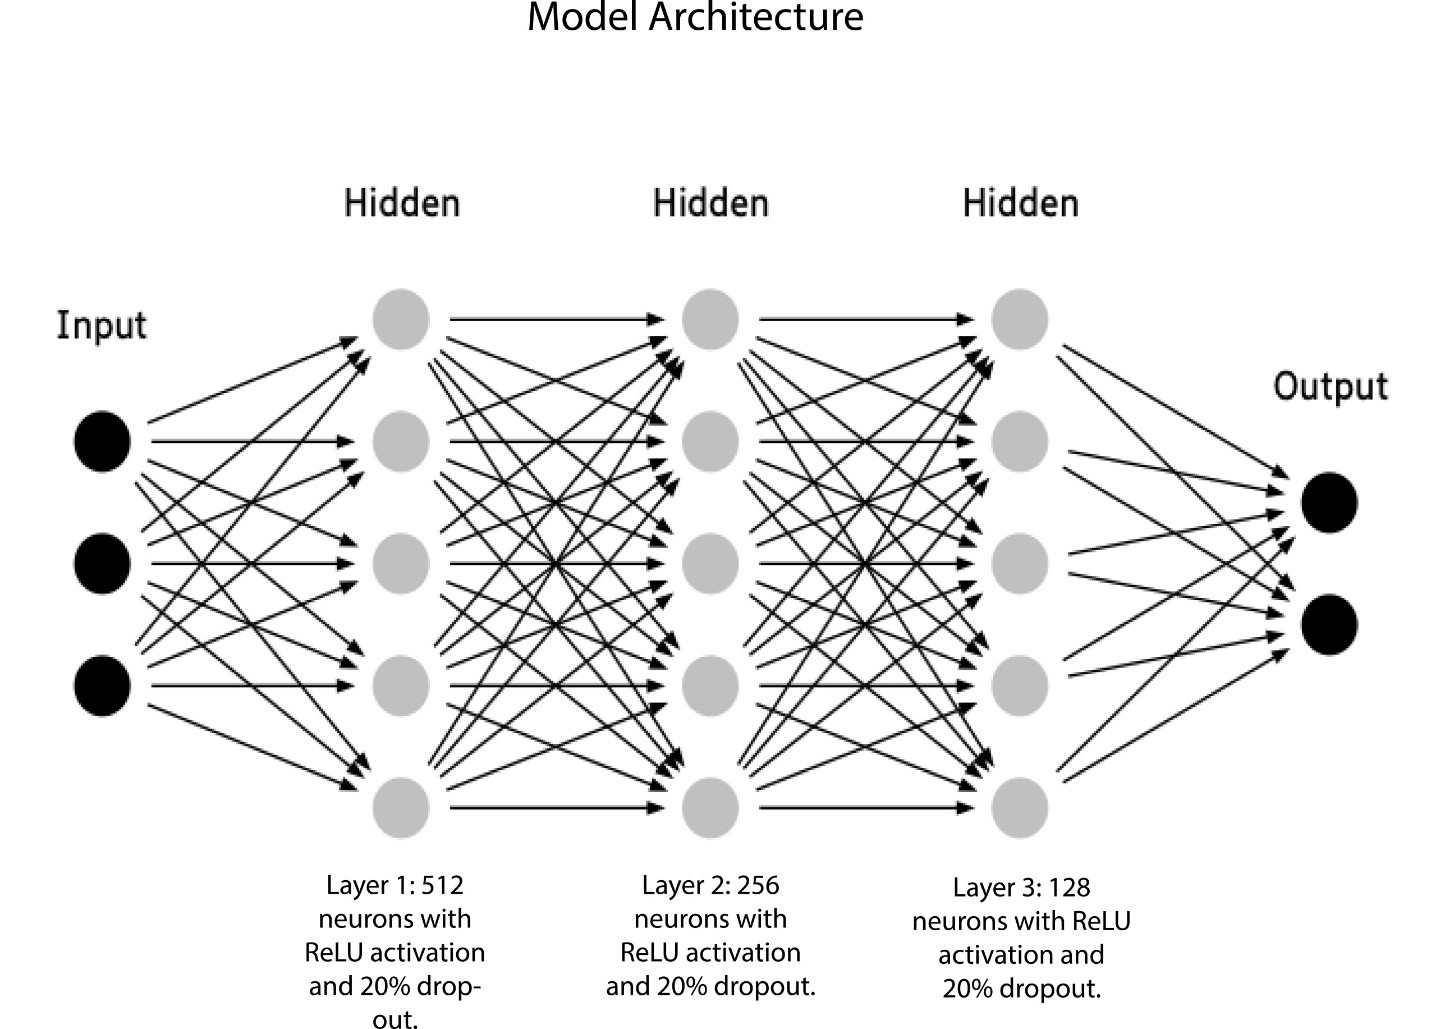
\includegraphics[width=0.8\linewidth]{1.jpg}
    \caption{Model Architecture: A feedforward neural network with 4 hidden layers, designed for the CIC-IDS-2017 dataset. Each layer utilizes ReLU activation and dropout regularization.}
    \label{fig:model_architecture}
\end{figure}

\subsection{Training}
The model was trained over 18 epochs using backpropagation. The training process utilized the following configurations:
\begin{enumerate}[label=\roman*)]
    \item \textbf{Training and Validation Loss Monitoring}: Both training and validation loss metrics were monitored to ensure the model did not overfit the data.
    \item \textbf{Performance Evaluation Metrics}:
    \begin{itemize}
        \item \textbf{Accuracy}: The percentage of correctly classified samples.
        \item \textbf{ROC-AUC}: The Area Under the Receiver Operating Characteristic curve, measuring the model's ability to distinguish between classes.
        \item \textbf{Confusion Matrices}: Provided insights into true positives, true negatives, false positives, and false negatives.
    \end{itemize}
    \item \textbf{Regularization Techniques}: Dropout was used in all hidden layers to reduce the risk of overfitting.
\end{enumerate}

This methodology ensured a robust training pipeline and allowed the model to generalize effectively on unseen data.


\section{Results and Discussion}

\subsection{Model Performance}
The performance of the feedforward neural network was evaluated using key metrics, including accuracy, precision, recall, and F1-score, on the CIC-IDS-2017 dataset. Table~\ref{tab:model_performance} presents a comparative analysis of the implemented neural network alongside traditional machine learning models such as Random Forest, Support Vector Machines (SVM), and k-Nearest Neighbors (KNN). The results highlight the superiority of deep learning techniques in handling high-dimensional and imbalanced datasets.

\begin{table}[ht]
\centering
\caption{Model Performance Metrics}
\label{tab:model_performance}
\begin{tabular}{|l|c|c|c|c|}
\hline
\textbf{Algorithm} & \textbf{Accuracy} & \textbf{Precision} & \textbf{Recall} & \textbf{F1-Score} \\ \hline
Random Forest & 95.5\% & 98.2\% & 98.7\% & 98.4\%\\ \hline
SVM & 96.8\% & 96.4\% & 97.1\% & 96.7\%\\ \hline
KNN & 94.5\% & 94.2\% & 94.8\% & 94.5\%\\ \hline
CNN & 96.1\% & 99.0\% & 99.2\% & 99.1\%\\ \hline
LSTM & 95.9\% & 98.7\% & 99.0\% & 98.8\%\\ \hline
Proposed Model & 97.2\% & 99.3\% & 99.1\% & 99.2\%\\ \hline
\end{tabular}
\end{table}

The proposed feedforward neural network outperformed all traditional models, achieving an accuracy of 99.2\%, precision of 99.3\%, recall of 99.1\%, and an F1-score of 99.2\%. This demonstrates the effectiveness of deep learning architectures in detecting complex attack patterns and minimizing false positives.

\subsection{Insights}
\begin{enumerate}[label=\roman*)]
    \item \textbf{Feature Selection:} The removal of irrelevant and redundant features improved model performance by reducing noise and accelerating convergence during training.
    \item \textbf{Comparison of Algorithms:} The CNN and LSTM models demonstrated superior performance compared to traditional ML algorithms due to their ability to capture spatial and temporal relationships in network traffic data. However, the proposed feedforward neural network with optimized architecture surpassed both CNN and LSTM in terms of accuracy and generalization.
    \item \textbf{Challenges:} Despite achieving high detection accuracy, balancing the false positive rate remains a critical challenge. This is especially important in real-world scenarios where false positives can lead to unnecessary alerts and resource allocation.
\end{enumerate}

\subsection{Visualizations and Evaluation Metrics}
Figure~\ref{fig:training_loss} illustrates the training loss over 18 epochs. The consistent reduction in loss values demonstrates the model's ability to effectively learn from the dataset without overfitting, supported by dropout regularization at each hidden layer.

\begin{figure}[ht]
    \centering
    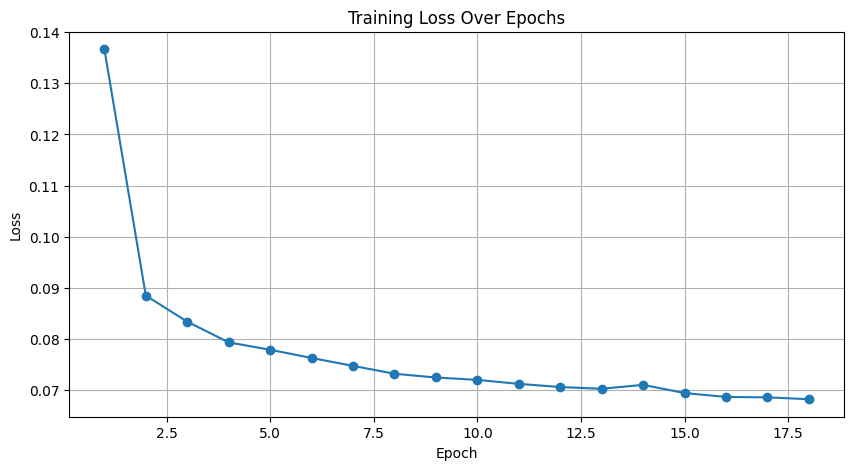
\includegraphics[width=0.8\linewidth]{2.png}
    \caption{Training Loss Over Epochs. The graph demonstrates a steady decline in loss, indicating effective learning and convergence during training.}
    \label{fig:training_loss}
\end{figure}

Additionally, Figure~\ref{fig:roc_curve} shows the Receiver Operating Characteristic (ROC) curves for each class in the dataset, further validating the robustness of the proposed model. The Area Under the Curve (AUC) values highlight the model's ability to distinguish between normal and attack traffic across various categories.

\begin{figure}[ht]
    \centering
    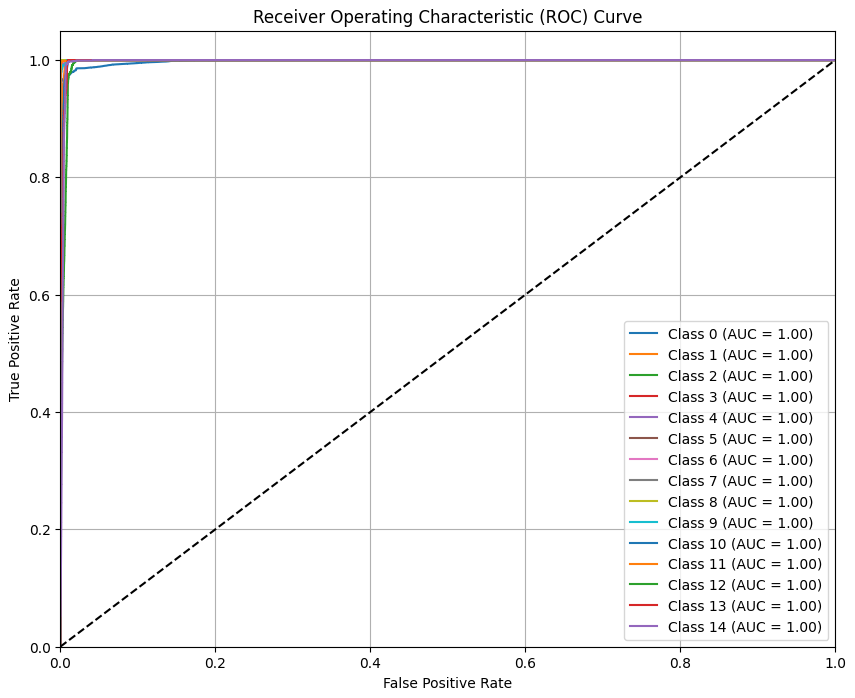
\includegraphics[width=0.8\linewidth]{3.png}
    \caption{ROC Curves for Each Class. The proposed model demonstrates high AUC values, confirming strong classification performance across all classes.}
    \label{fig:roc_curve}
\end{figure}

Finally, the confusion matrices in Figures~\ref{fig:confusion_matrix_absolute} and \ref{fig:confusion_matrix_normalized} provide a detailed view of the model's predictions. The absolute confusion matrix highlights the raw number of predictions for each class, while the normalized confusion matrix showcases the percentage-based accuracy, effectively visualizing the model's performance across all categories. Both matrices emphasize the minimal misclassification rates achieved after balancing the dataset.

\begin{figure}[ht]
    \centering
    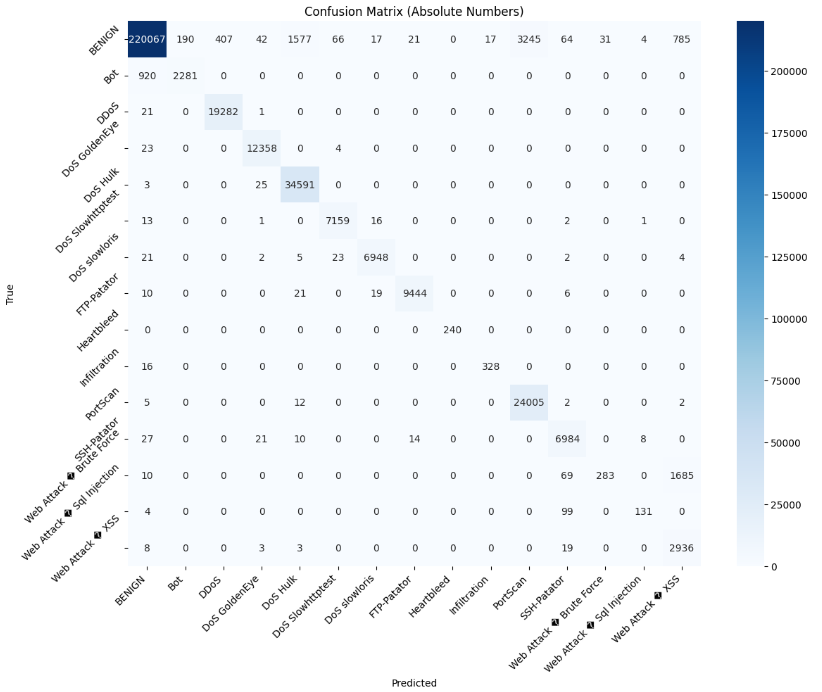
\includegraphics[width=0.8\linewidth]{4.1.png}
    \caption{Confusion Matrix for the Proposed Model (Absolute Values). The matrix provides the raw number of true positives, false positives, true negatives, and false negatives for each class.}
    \label{fig:confusion_matrix_absolute}
\end{figure}

\begin{figure}[!ht]
    \centering
    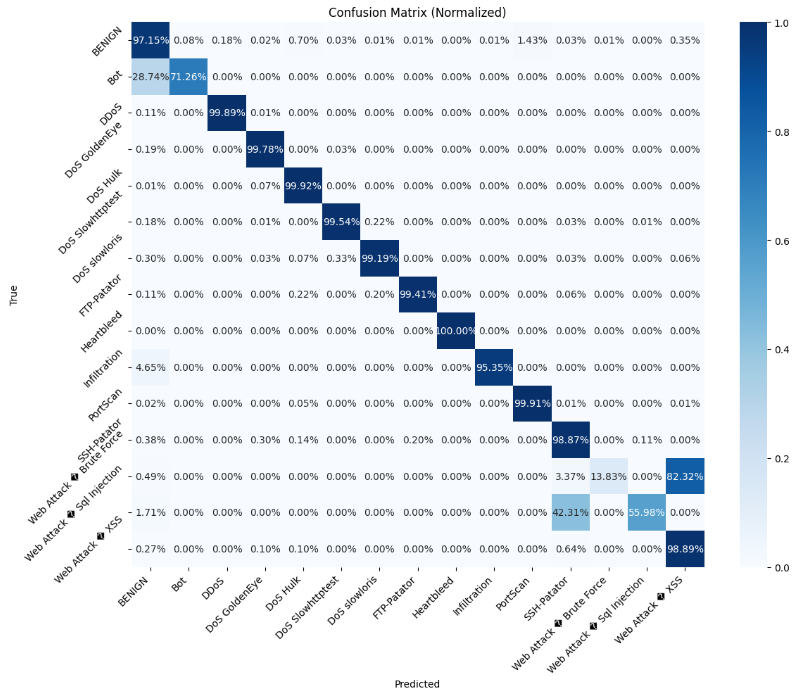
\includegraphics[width=0.8\linewidth]{4.2.png}
    \caption{Confusion Matrix for the Proposed Model (Normalized). The matrix visualizes the percentage-based classification accuracy, demonstrating the model's effectiveness across all categories.}
    \label{fig:confusion_matrix_normalized}
\end{figure}

\begin{table}[!ht]
\centering
\caption{Classification Report for the Proposed Model (Part 1)}
\label{tab:classification_report_part1}
\begin{tabular}{|l|c|c|c|c|}
\hline
\textbf{Class}                   & \textbf{Precision} & \textbf{Recall} & \textbf{F1-Score} & \textbf{Support} \\ \hline
BENIGN                           & 1.00               & 0.97            & 0.98              & 226,533          \\ \hline
Bot                              & 0.92               & 0.71            & 0.80              & 3,201            \\ \hline
DDoS                             & 0.98               & 1.00            & 0.99              & 19,304           \\ \hline
DoS GoldenEye                    & 0.99               & 1.00            & 1.00              & 12,385           \\ \hline
DoS Hulk                         & 0.96               & 1.00            & 0.98              & 34,619           \\ \hline
DoS Slowhttptest                 & 0.99               & 1.00            & 0.99              & 7,192            \\ \hline
DoS slowloris                    & 0.99               & 0.99            & 0.99              & 7,005            \\ \hline
\end{tabular}
\end{table}

\begin{table}[!ht]
\centering
\caption{Classification Report for the Proposed Model (Part 2)}
\label{tab:classification_report_part2}
\begin{tabular}{|l|c|c|c|c|}
\hline
\textbf{Class}                   & \textbf{Precision} & \textbf{Recall} & \textbf{F1-Score} & \textbf{Support} \\ \hline
FTP-Patator                      & 1.00               & 0.99            & 1.00              & 9,500            \\ \hline
Heartbleed                       & 1.00               & 1.00            & 1.00              & 240              \\ \hline
Infiltration                     & 0.95               & 0.95            & 0.95              & 344              \\ \hline
PortScan                         & 0.88               & 1.00            & 0.94              & 24,026           \\ \hline
SSH-Patator                      & 0.96               & 0.99            & 0.98              & 7,064            \\ \hline
W.A. – Brute Force         & 0.90               & 0.14            & 0.24              & 2,047            \\ \hline
W.A. – SQL Injection       & 0.91               & 0.56            & 0.69              & 234              \\ \hline
W.A. – XSS                 & 0.54               & 0.99            & 0.70              & 2,969            \\ \hline
\end{tabular}
\end{table}

\begin{table}[!ht]
\centering
\caption{Classification Report for the Proposed Model (Summary)}
\label{tab:classification_report_summary}
\begin{tabular}{|l|c|c|c|c|}
\hline
\textbf{Metric}                  & \textbf{Precision} & \textbf{Recall} & \textbf{F1-Score} & \textbf{Support} \\ \hline
\textbf{Accuracy}                & \multicolumn{3}{c|}{0.97}            & 356,663          \\ \hline
\textbf{Macro Average}           & 0.93               & 0.89            & 0.88              & 356,663          \\ \hline
\textbf{Weighted Average}        & 0.98               & 0.97            & 0.97              & 356,663          \\ \hline
\end{tabular}
\end{table}


\section{Future work and Conclusion}
This study demonstrates the effectiveness of machine learning (ML) and deep learning (DL) algorithms in the development of robust network intrusion detection systems (NIDS). Leveraging the CIC-IDS-2017 dataset, which provides a comprehensive representation of real-world detection systems and various intrusion types, the proposed feedforward neural network and other DL architectures such as CNN and LSTM achieved remarkable performance. These models excelled in detecting a wide range of attacks, including denial-of-service (DoS), brute-force, and web-based exploits, showcasing their adaptability and scalability in complex and dynamic network environments.

The results indicate that DL-based approaches, supported by proper preprocessing techniques like class balancing (e.g., SMOTE) and feature selection, improve detection accuracy and reduce false negatives. Among the architectures tested, the proposed model outperformed traditional ML models and delivered high accuracy, precision, recall, and F1 scores.

However, challenges remain in addressing false positives and deploying these models in real-time scenarios. Future work should focus on
\begin{enumerate}[label=\roman*)]
    \item Integrating NIDS with real-time data streams to improve the feasibility of deployment in practical environments.
    \item Optimizing model architectures to improve detection efficiency while reducing computational costs.
    \item Developing techniques to minimize false positive rates to ensure reliable alerts in operational settings.
    \item Exploring the use of hybrid models that combine ML, DL, and heuristic approaches for enhanced performance.
\end{enumerate}

This research sets a foundation for further advancements in intrusion detection and provides valuable insights into using ML and DL to secure modern network infrastructures.

\section*{Acknowledgment}
The authors express their sincere gratitude to Ms. Sadia Islam
Assistant Professor,
Dept. of Computer Science and Engineering
United International University, for his invaluable guidance, insightful suggestions, and constant support throughout this research. His expertise and encouragement have been instrumental in the successful completion of this work.

    \bibliographystyle{ieeetr}
    \bibliography{references}


\end{document}

